\documentclass[UTF8]{ctexart}
\usepackage[a4paper, top=25.4mm, bottom=25.4mm, left=31.8mm, right=31.8mm]{geometry}
\usepackage{graphicx}
\usepackage{amsmath}
\usepackage{multirow}
\usepackage{listings}
\usepackage{subcaption}
\usepackage{tabu}
\usepackage[T1]{fontenc}
\usepackage{booktabs}
\usepackage{minted}
\usemintedstyle{manni}
\usepackage[table]{xcolor}

\setlength{\parskip}{1em}
\definecolor{lightergray}{gray}{0.95}
\setlength{\tabcolsep}{12pt}
\renewcommand{\arraystretch}{1}
\lstset{
basicstyle=\ttfamily,
columns=flexible,
breaklines=true
}

\begin{document}
\begin{titlepage}
  \begin{center}
    \vspace*{1cm}

    \Large
    编译原理

    \vspace{0.5cm}
    \Huge
    \textbf{语法分析实验实验报告}

    \vfill

    \normalsize\kaishu
    班级:07111603 \\
    学号:1120161730 \\
    姓名:武上博 \\
    \today
    \vspace{1cm}
  \end{center}
\end{titlepage}

\tableofcontents
\newpage

\section{实验目的}
\begin{enumerate}
  \item 熟悉 C 语言的语法规则,了解编译器语法分析器的主要功能
  \item 熟练掌握典型语法分析器构造的相关技术和方法,设计并实现具有一定分析能力的 C 语言语法分析器
  \item 掌握编译器从前端到后端各个模块的工作原理,语法分析模块与其他模块之间的交互过程
\end{enumerate}

\section{实验内容}
\begin{enumerate}
  \item 该实验选择 C 语言的一个子集,基于 BIT-MiniCC 构建 C 语法子集的语法分析器,该语法分析器能够读入 XML 文件形式的属性字符流,进行语法分析并进行错误处理,如果输入正确时输出 XML 形式的语法树,输入不正确时报告语法错误。
  \item 将分析树转换为抽象语法树,便于后续分析工作和代码生成工作的完成。
\end{enumerate}

\section{实验的具体过程步骤}
\subsection{项目整体架构设计}
本次语法分析实验是在上一个词法分析实验的基础之上进行的,我们的大致要求是将词法分析得到的 Token 文件读入,作为语法分析的输入串,在通过语法分析器之后得到相应的语法树。经过考虑,我决定使用自顶向下的 LL(1) 语法分析方法。

LL(1) 语法分析器的具体架构是这样的:

\begin{itemize}
  \item 文法输入模块
  \item LL(1) 主控程序
  \begin{itemize}
    \item First 集合求解模块
    \item Follow 集合求解模块
    \item LL(1) 分析表构造模块
  \end{itemize}
  \item 输入串分析模块
\end{itemize}

为了和 BIT-MiniCC 框架进行结合,我们需要读入词法分析 Token 的 XML 文件作为我们的输入。同时我们需要输出符合规范的抽象语法树对应的 XML 文件作为下一步的输入。

我本次项目选择使用 Python 进行实现。我设计了:

\begin{itemize}
  \item \texttt{main.py}:LL(1) 分析器的主控程序,调用下面两个模块
  \item \texttt{parserUtils.py}:LL(1) 分析器的工具类,包含了对文法的读入、分析、First 和 Follow 集合的求取以及 LL(1) 分析表的求取等工具
  \item \texttt{parserGeneral.py}:LL(1) 分析器的主要模块,通过读入 Token 文件以及 LL(1) 分析表,得到语法分析树,并输出为合法的 XML 文件
\end{itemize}

这三个主要模块,构成了全部的 LL(1) 分析器。程序大致的流程如下图 \ref{fig:figure1}:

\begin{figure}[h]
  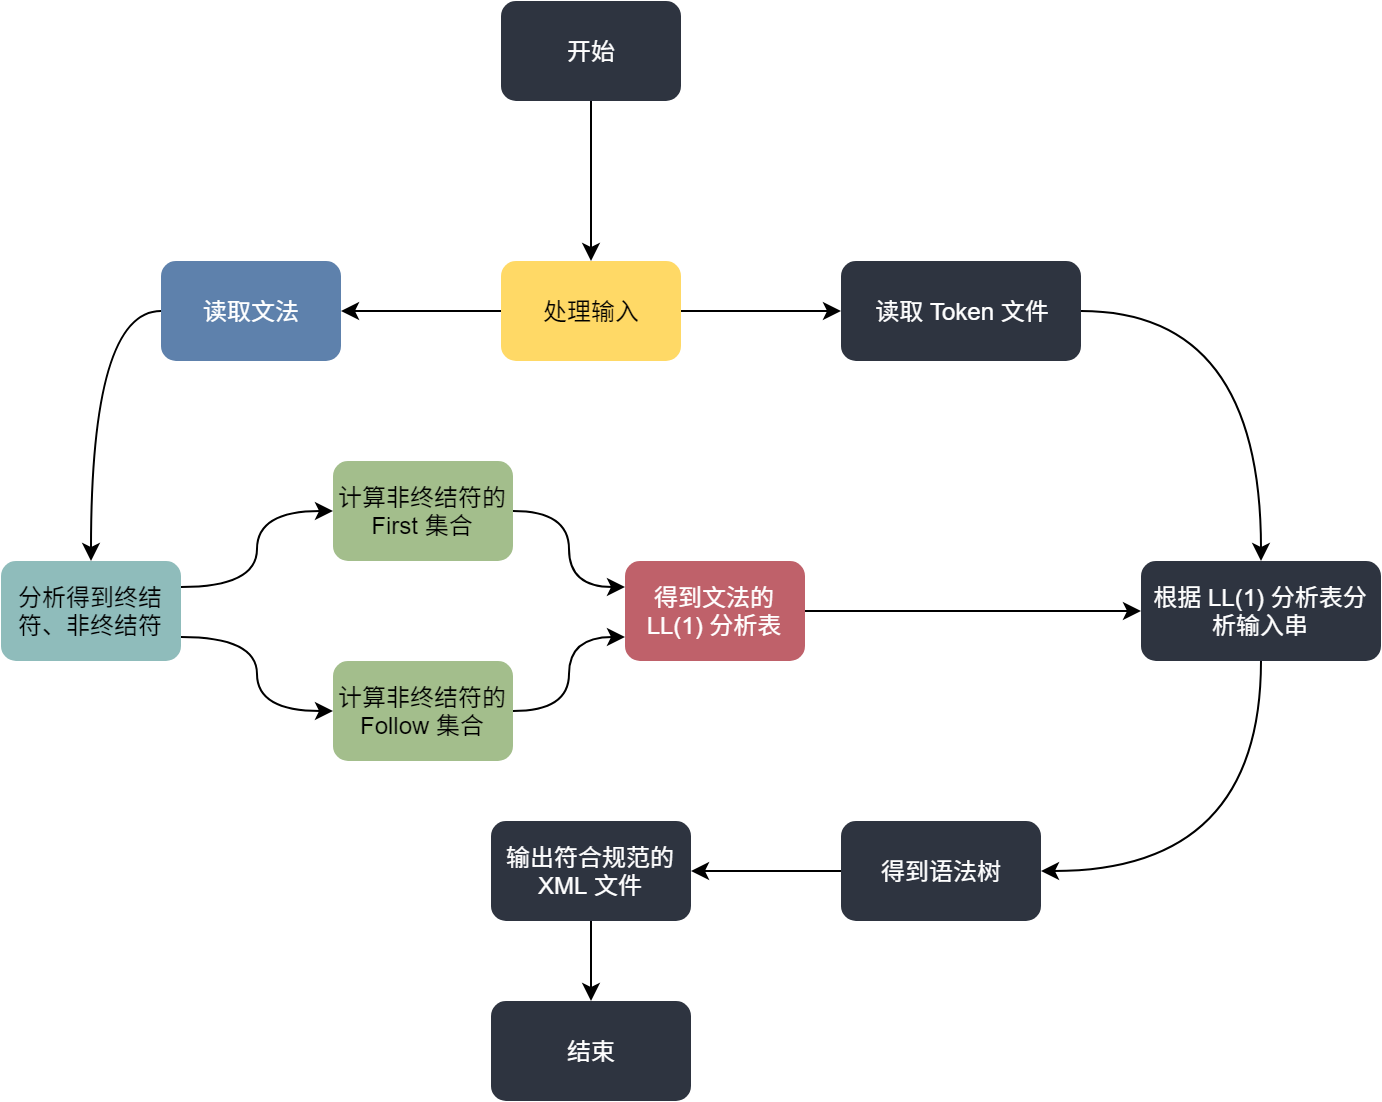
\includegraphics[width=\linewidth]{images/ll1.png}
  \caption{LL(1) 分析器的大致工作流程}
  \label{fig:figure1}
\end{figure}

\subsection{各个模块的具体实现}
接下来,我对每个模块的具体实现一一进行介绍。

\subsubsection{定义文法}
本次实验中,我在实验要求的文法基础之上,进行了一些扩展,增加了 C 语言中“声明语句”、“循环语句”、“判断语句”以及“跳转语句”的定义。同时,我也适当修改了原有的文法,包括对变量的声明、外部函数等等内容。本次实验中我所采用的全部文法如下所示:

\begin{lstlisting}
TRANSLATION_UNIT -> FUNCTION_DEFINITION
FUNCTION_DEFINITION -> TYPE_SPECIFIER identifier ( PARAM_LIST ) CODE_BLOCK
PARAM_LIST -> ARGUMENT | ARGUMENT , PARAM_LIST | empty
ARGUMENT -> TYPE_SPECIFIER identifier
TYPE_SPECIFIER -> int | float | short | long | void | double | char
CODE_BLOCK -> { STATEMENT_LIST }
STATEMENT_LIST -> STATEMENT STATEMENT_LIST | empty
STATEMENT -> DECLARATION_STATEMENT | ASSIGN_STATEMENT | RETURN_STATEMENT | LOOP_STATEMENT | SELECT_STATEMENT
DECLARATION_STATEMENT -> TYPE_SPECIFIER identifier ; | TYPE_SPECIFIER ASSIGN_STATEMENT
ASSIGN_STATEMENT -> identifier ASSIGN_OPERATOR EXPRESSION ;
ASSIGN_OPERATOR -> = | += | -= | *= | /= | ^= | %= | &=
RETURN_STATEMENT -> return EXPRESSION ;
JUMP_STATEMENT -> continue ; | break ; | goto identifier ;
LOOP_STATEMENT -> for ( EXPRESSION ; EXPRESSION ; EXPRESSION ) CODE_BLOCK | while ( EXPRESSION ) CODE_BLOCK | do CODE_BLOCK while ( EXPRESSION ) ;
SELECT_STATEMENT -> if ( EXPRESSION ) CODE_BLOCK | if ( EXPRESSION ) CODE_BLOCK else CODE_BLOCK | switch ( EXPRESSION ) CODE_BLOCK
EXPRESSION -> TERM EXPRESSION2 | empty
EXPRESSION2 -> + TERM EXPRESSION2 | - TERM EXPRESSION2 | empty
TERM -> FACTOR TERM2
TERM2 -> * FACTOR TERM2 | / FACTOR TERM2 | empty
FACTOR -> identifier | CONSTANT | ( EXPRESSION )
CONSTANT -> integer_constant | floating_constant | char | string
\end{lstlisting}

\subsubsection{输入文法,并以字典的形式存储}
为了方便存储文法,以 \texttt{FACTOR -> identifier | CONSTANT | (EXPRESSION)} 为例子,我按照如下的形式存储文法:

\begin{verbatim}
{
  'FACTOR': [['identifier'], ['CONSTANT'], ['(', 'EXPRESSION', ')']}
}
\end{verbatim}

可以看到,我将文法产生式左侧非终结符作为字典的 key,将相应的 value 定为文法后缀的生成式列表。我以 “\texttt{|}” 区分不同的生成式,这样就能够很好的对文法进行分析处理了。

相应的,在 Python 中,我使用了下面的方式对文法 \texttt{grammar} 进行初始化:

\begin{minted}[linenos,frame=lines,framesep=2mm]{python}
grammar = collections.defaultdict(list)
\end{minted}

之后,按行读入文法,并处理,最后得到“字典嵌套列表”的一个数据结构。

\begin{minted}[linenos,frame=lines,framesep=2mm]{python}
with open(filePath, 'r') as f:
    # 按行读取,加入文法字典
    for line in f:
      preGrammar, postGrammar = line.rstrip('\n').split('->')
      preGrammar = preGrammar.rstrip(' ')
      postGrammar = postGrammar.lstrip(' ').split('|')

      for eachPostGrammar in postGrammar:
        eachPostGrammar = eachPostGrammar.strip(' ').split(' ')
        grammar[preGrammar].append(eachPostGrammar)
\end{minted}

\subsubsection{处理终结符与非终结符}
对输入的文法进行遍历获取终结符与非终结符列表相对简单,只需要将文法生成式的前部加入非终结符集合,再遍历文法的后缀,如果遇到了不在非终结符集合中的符号,直接加入终结符集合即可。

\begin{minted}[linenos,frame=lines,framesep=2mm]{python}
def differentiateSymbols(grammar):
  # ...
  return terminalSymbols, nonTerminalSymbols
\end{minted}

通过上面两个步骤,我们已经成功的得到了文法的具体内容、文法的终结符与非终结符集合。这样,我们就可以利用这三个集合,通过接下来的算法构造 LL(1) 分析表。

\subsubsection{获取文法的 First 与 Follow 集合}
\paragraph{First 集合}
首先,我们对文法的每一项非终结符求取其 First 集合。First 集合是非终结符(或终结符、空符号串等等)的开始符号集合。对于文法 G 来说,G 中的 $\forall \alpha \in V^*$ 终结首符号集合 $FIRST(\alpha)$ 为:

\begin{equation}
  FIRST(\alpha) = \{a | \alpha^* \implies a, a \in V_T\}
\end{equation}

若 $a^* \implies \epsilon$,则 $\epsilon \in FIRST(\alpha)$。

在求取 First 集合时,我们是通过下面大致的代码描述进行求取的。

\begin{minted}[linenos,frame=lines,framesep=2mm]{python}
def getFIRST(firstSet, grammar, terminalSymbols, nonTerminalSymbols):
  for eachGrammar in grammar:
    for eachPostGrammar in grammar[eachGrammar]:
      # 1. 遇到了终结符、产生式右侧子式首符号是终结符,直接加入
      if ...
      # 2. 产生式右侧子式首符号,递归求取(比如:A -> B C c)
      else ...
  return firstSet
\end{minted}

为了保证 First 集合的完整性,我们需要递归多次求取文法的 First 集合。在主控程序循环求取 First 集合,直到两次求得的 First 集合相同即可停止。

\begin{minted}[linenos,frame=lines,framesep=2mm]{python}
grammarFirstSet = collections.defaultdict(list)
grammarFirstSet = parserUtils.getFIRST(
    grammarFirstSet, grammar, terminalSymbols, nonTerminalSymbols)
while True:
  originalFirstSet = copy.deepcopy(grammarFirstSet)
  grammarFirstSet = parserUtils.getFIRST(
      grammarFirstSet, grammar, terminalSymbols, nonTerminalSymbols)
  if grammarFirstSet == originalFirstSet:
    break
\end{minted}

\paragraph{Follow 集合}
在上一步骤 First 集合的基础之上,我们求取 Follow 集合。Follow 集合是对于文法 G 的所有句型中能够紧跟在非终结符号后面的一切终结符号(或者“\#”)。对上下文无关文法 G 来说,S 是文法的开始符号,对于文法 G 的任何非终结符号 A:

\begin{equation}
  FOLLOW(A) = \{ a | S^* \implies \dots Aa \dots, a \in V_T^* \}
\end{equation}

若 $S^* \implies \dots A$,则 $\# \in FOLLOW(A)$。

我们在构造 Follow 集合时,采用下面描述的算法:

\noindent\fbox{%
  \parbox{\linewidth}{%
对文法 G 中每个 $A \in V_N$:

\begin{enumerate}
  \item 对 G 的开始符号 S,令 $\# \in FOLLOW(S)$
  \item 如果文法 G 中出现了形如 $B \rightarrow \alpha A\beta$ 的产生式,且 $\beta \neq \epsilon$,则将 $FIRST(\beta)$ 中除了 $\epsilon$ 的符号全部加入 FOLLOW(A) 中
  \item 如果文法 G 中出现了形如 $B \rightarrow \alpha A$,或 $B \rightarrow \alpha A \beta$ 且 $\epsilon \in FIRST(\beta)$ 的产生式,则将 FOLLOW(B) 中全部内容加入 FOLLOW(A) 中
\end{enumerate}
  }%
}

在具体的代码实现中:

\begin{minted}[linenos,frame=lines,framesep=2mm]{python}
def getFOLLOW(firstSet, followSet, grammar, terminalSymbols, nonTerminalSymbols):
  for eachGrammarStartSymbol in grammar.keys():
    for eachGrammar in grammar:
      for eachPostGrammar in grammar[eachGrammar]:
        if eachGrammarStartSymbol in eachPostGrammar:
          # 1. 产生式形如:S->aX,将集合 Follow(S) 中的所有元素加入 Follow(X) 中
          if ...
          # 2. 产生式形如:S->aXb
          else ...
            # 2.1 b 为终结符:将 b 加入 Follow(X) 中
            if ...
            # 2.2 b 为非终结符
            else ...
  return followSet
\end{minted}

\subsubsection{得到相应的 LL(1) 分析表}

\subsubsection{处理输入 Token,得到分析树}

\section{运行效果}
\subsection{语法树的生成}

\subsection{得到抽象语法树的 XML 表示}

\section{实验心得体会}
通过本次实验,我不仅更加熟悉了语法分析的具体过程,对自上而下的语法分析过程更加了解,还对 C 语言的文法描述、LL(1) 分析法的具体过程以及通过 LL(1) 分析表处理输入串的过程有了全新的认识。我在本次实验中,通过自己的扩展,处理得到了一个相对清晰的 C 语言 LL(1) 文法子集,利用 Python 构建了 C 语言的语法分析器,并成功的通过 LL(1) 分析器得到了一段 C 语言代码的语法分析树。

在本次实验中,我遇到最大的难题是对文法的处理。只有选取合适的数据结构,我才能更加方便的处理 C 语言的文法集合,也更加方便后续利用 LL(1) 分析表构建语法分析树的遍历过程。

与此同时,我通过本次实验的学习,还对 LL(1) 语法分析法、递归下降分析法以及 LR 语法分析法都有了全新的了解。总体来说,我收获颇丰。

\end{document}